\documentclass[12pt]{article}
\usepackage{amsmath}
\usepackage{amssymb}
\usepackage[letterpaper,top=1.2in,bottom=1in,left=0.75in,right=0.75in,centering]{geometry}
%\usepackage{fancyhdr}
\usepackage{enumerate}
%\usepackage{lastpage}
\usepackage{multicol}
\usepackage{graphicx}

\reversemarginpar

%\pagestyle{fancy}
%\cfoot{}
%\lhead{Math 1560}\chead{Test \# 1}\rhead{May 18th, 2017}
%\rfoot{Total: 10 points}
%\chead{{\bf Name:}}
\newcommand{\points}[1]{\marginpar{\hspace{24pt}[#1]}}
\newcommand{\skipline}{\vspace{12pt}}
%\renewcommand{\headrulewidth}{0in}
\headheight 30pt

\newcommand{\di}{\displaystyle}
\newcommand{\abs}[1]{\lvert #1\rvert}
\newcommand{\len}[1]{\lVert #1\rVert}
\renewcommand{\i}{\mathbf{i}}
\renewcommand{\j}{\mathbf{j}}
\renewcommand{\k}{\mathbf{k}}
\newcommand{\R}{\mathbb{R}}
\newcommand{\aaa}{\mathbf{a}}
\newcommand{\bbb}{\mathbf{b}}
\newcommand{\ccc}{\mathbf{c}}
\newcommand{\dotp}{\boldsymbol{\cdot}}
\newcommand{\bbm}{\begin{bmatrix}}
\newcommand{\ebm}{\end{bmatrix}}       
\newcommand{\bvm}{\begin{vmatrix}}
\newcommand{\evm}{\end{vmatrix}}       
\DeclareMathOperator{\proj}{proj}            
                  
\begin{document}


\author{Instructor: Sean Fitzpatrick}
\thispagestyle{empty}
\vglue1cm
\begin{center}
{\bf MATH 1410 - Tutorial \#4 Solutions}
\end{center}

\textbf{Additional practice:}
\begin{enumerate}
\item Find the equation of the line through the point $(1,-2,4)$ that is parallel to the line
\[
\langle x,y,z\rangle = \langle 3-4t,2+t,5\rangle.
\]

The given line has direction vector $\langle -4,1,0\rangle$. Our line should have the same direction vector but pass through $(1,-2,4)$, so the equation is
\[
\langle x,y,z\rangle = \langle 1-4t,-2+t,4\rangle.
\]
\item Find the area of the parallelogram with vertices $(1,2,3), (4,0,7), (0,3,5)$, and $(3,1,9)$.

\medskip

Labelling the vertices $P,Q,R,S$, respectively, we find
\[
\overrightarrow{PQ}=\langle 3,-2,4\rangle \text{ and } \overrightarrow{PR}=\langle -1,1,2\rangle.
\]
However, we need to check to make sure that the vertices $Q$ and $R$ are adjacent to $P$. Since we have $\overrightarrow{RS}=\langle 3,-2,4\rangle=\overrightarrow{PQ}$, we know that the vectors $\overrightarrow{PQ}$ and $\overrightarrow{RS}$ represent opposite sides of the parallelogram, and $S$ is the vertex not adjacent to $P$.

We now compute
\[
\overrightarrow{PQ}\times \overrightarrow{PR} = \bvm -2&4\\1&2\evm\i-\bvm 3&4\\-1&2\evm\j +\bvm 3&-2\\-1&1\evm\k = \langle -8,-10,1\rangle,
\]
so the area is given by
\[
A = \len{\overrightarrow{PQ}\times \overrightarrow{PR}} = \sqrt{8^2+10^2+1^2}=\sqrt{165}.
\]
\item Prove \textit{Lagrange's identity}: for any vectors $\vec{a},\vec{b}$ in $\R^3$, $\len{\vec{a}}^2\len{\vec{b}}^2=\len{\vec{a}\times\vec{b}}^2 +(\vec{a}\dotp\vec{b})^2.$

Let $\vec{a} = \langle a_1,a_2,a_3\rangle$ and $\vec{b}=\langle b_1,b_2,b_3\rangle$. Then
\[
\vec{a}\times\vec{b} = \langle a_2b_3-a_3b_2,a_3b_1-a_1b_3,a_1b_2-a_2b_1\rangle
\]
and
\[
\vec{a}\dotp\vec{b} = a_1b_1+a_2b_2+a_3b_3,
\]
so
\begin{align*}
\len{\vec{a}\times\vec{b}}^2 &= (a_2b_3-a_3b_2)^2+(a_3b_1-a_1b_3)^2+(a_1b_2-a_2b_1)^2\\
&=a_1^2b_2^2+a_1^2b_3^2+a_2^2b_1^2+a_2^2b_3^2+a_3^2b_1^2+a_3^2b_2^2-2(a_1a_2b_1b_2+a_1a_3b_1b_3+a_2a_3b_2b_3),
\end{align*}
and
\begin{align*}
(\vec{a}\dotp\vec{b})^2 & = (a_1b_1+a_2b_2+a_3b_3)^2\\
& = a_1^2b_1^2+a_2^2b_2^2+a_3^2b_3^2 +2(a_1b_1a_2b_2+a_1b_1a_3b_3+a_2b_2a_3b_3).
\end{align*}
Adding these together, we see that second terms in each of the above equations cancel, giving us
\begin{align*}
\len{\vec{a}\times\vec{b}}^2+(\vec{a}\dotp\vec{b})^2 &= a_1^2b_2^2+a_1^2b_3^2+a_2^2b_1^2+a_2^2b_3^2+a_3^2b_1^2 +a_3^2b_2^2+a_1^2b_1^2+a_2^2b_2^2+a_3^2b_3^2\\
&=(a_1^2+a_2^2+a_3^2)(b_1^2+b_2^2+b_3^2)\\
& = \len{\vec{a}}^2+\len{\vec{b}}^2,
\end{align*}
as required.

\item Prove that if $\vec{a}$ is parallel to $\vec{b}$, then $\vec{a}\times\vec{b}=\vec{0}$. You may use the properties of the cross product given in Theorem 17 on page 80 of the textbook.

\bigskip

If $\vec{a}$ is parallel to $\vec{b}$, then $\vec{b}=k\vec{a}$ for some scalar $k$. (If we consider the zero vector to be parallel to any vector, we could include this as a degenerate case, but if one of the two vectors is zero, so is the cross product.) Using properties of the cross product, we then have
\[
\vec{a}\times \vec{b} = \vec{a}\times (k\vec{a}) = k(\vec{a}\times\vec{a})=k\vec{0}=\vec{0},
\]
since the cross product of any vector with itself is zero.

\medskip

\item Determine the point of intersection (if any) of the lines
\[
\ell_1(s)  = \langle 5,3,0\rangle + s\langle 3,1,-2\rangle\quad\text{ and } \quad
\ell_2(t)  = \langle -2,4,4\rangle+t\langle 1,-3,0\rangle
\]

\medskip

If $(x,y,z)$ is a point of intersection, then we must have
\begin{align*}
x&=5+3s=-2+t\\
y&=3+s=4-3t\\
z&=-2s=4,
\end{align*}
since the point is on both lines, and must therefore satisfy both equations. Looking at the $z$ coordinate, we must have $s=-2$. Putting this value in for the $y$ coordinate gives us
$3-2=1=4-3t$, so $-3t=1-4=-3$, giving $t=1$. We now check whether these values both work for the $x$ coordinate: $5+3(-2)=-1$, and $-2+1=-1$, so putting $s=-2$ in the first line gives us the point $(-1,1,4)$, and putting $t=1$ into the second line gives the same point, so the point $(-1,1,4)$ must be the point of intersection.

\end{enumerate}


\newpage
%\thispagestyle{empty}

\textbf{Assigned problems:}
\begin{enumerate}

  
 \item Find the area of the triangle with vertices $P=(2,0,-1)$, $Q=(-3,4,2)$, and $R=(0,-3,1)$.

\bigskip

Consider the vectors
\begin{align*}
 \vec{u} &= \overrightarrow{PQ}=\langle -5,4,3\rangle \text{ and}\\
 \vec{v} &= \overrightarrow{PR}=\langle -2,-3,2\rangle.
\end{align*}
We know that the area of the parallelogram spanned by $\vec{u}$ and $\vec{v}$ is given by $\len{\vec{u}\times\vec{v}}$, and the given triangle is exactly half of this parallelogram. Since
\begin{align*}
 \vec{u}\times\vec{v} &= \bvm 4&3\\-3&2\evm\hat{\imath}-\bvm -5&3\\-2&2\evm\hat{\jmath}+\bvm -5&4\\-2&-3\evm\hat{k}\\[3pt]
 & = (4(2)-3(-3))\hat{\imath}-(-5(2)-3(-2))\hat{\jmath}+(-5(-3)-4(-2))\hat{k}\\
 & = 17\hat{\imath}+4\hat{\jmath}+23\hat{k} = \langle 17,4,23\rangle,
\end{align*}
we have
\[
 A = \frac{1}{2}\len{\vec{u}\times\vec{v}}=\frac{1}{2}\sqrt{(17)^2+4^2+(23)^2}.
\]


\item Find the equation of the line that passes through the points $P=(2,-1,4)$ and $Q=(-1,3,2)$.

\bigskip

We know that a vector in the direction of the line is given by
\[
\vec{v}=\overrightarrow{PQ}=\langle -3,4,-2\rangle.
\]
Choosing $P=(2,-1,4)$ as our reference point on the line, we have the vector equation
\[
\langle x,y,z\rangle = \langle 2,-1,4\rangle+t\langle -3,4,-2\rangle = \langle 2-3t, -1+4t, 4-2t\rangle
\]
as the equation of the line.

 \item Show that for any two vectors $\vec{a},\vec{b}$ in $\R^3$, $\vec{a}$ is orthogonal to $\vec{a}\times\vec{b}$.
 
 \bigskip
 
 Let $\vec{a}=\langle a_1,a_2,a_3\rangle$ and $\vec{b} = \langle b_1,b_2,b_3\rangle$. Then
 \begin{align*}
 \vec{a}\dotp (\vec{a}\times\vec{b}) & = \langle a_1,a_2,a_3\rangle\dotp \langle a_2b_3-a_3b_2,a_3b_1-a_1b_3,a_1b_2-a_2b_1\rangle\\
 & = a_1(a_2b_3-a_3b_2)+a_2(a_3b_1-a_1b_3)+a_3(a_1b_2-a_2b_1)\\
 & = (a_1a_2b_3-a_1a_3b_2)+(a_2a_3b_1-a_2a_1b_3)+(a_3a_1b_2-a_3a_2b_1)\\
 & = (a_1a_2b_3-a_2a_1b_3)+(a_2a_3b_1-a_3a_2b_1)+(a_3a_1b_2-a_1a_3b_2)\\
 & = 0+0+0=0.
 \end{align*}
 Since the dot product is zero, the two vectors are orthogonal.

\newpage

\item Find the shortest distance from the point $P=(1,3,-2)$ to the line through the point $P_0 = (2,0,-1)$ in the direction of $\vec{v} = \langle 1, -1, 0\rangle$. Also find the point $P_1$ on the line that is closest to $P$. {\bf Include a diagram.}


\bigskip

\begin{multicols}{2}
 We label a generic diagram as shown to the right, with the points $P_0$, $P_1$ on the line labelled, as well as the point $P$ not on the line. From the diagram, we can see that the projection of the vector $\overrightarrow{P_0P}$ onto the line (which is the same as the projection of $\overrightarrow{P_0P}$ onto the vector $\vec{v}$, since $\vec{v}$ is parallel to the line) gives us the vector $\overrightarrow{P_0P_1}$: we have $\overrightarrow{P_0P_1} = \proj_{\vec{v}}\overrightarrow{P_0P}$.
\columnbreak

\begin{center}
 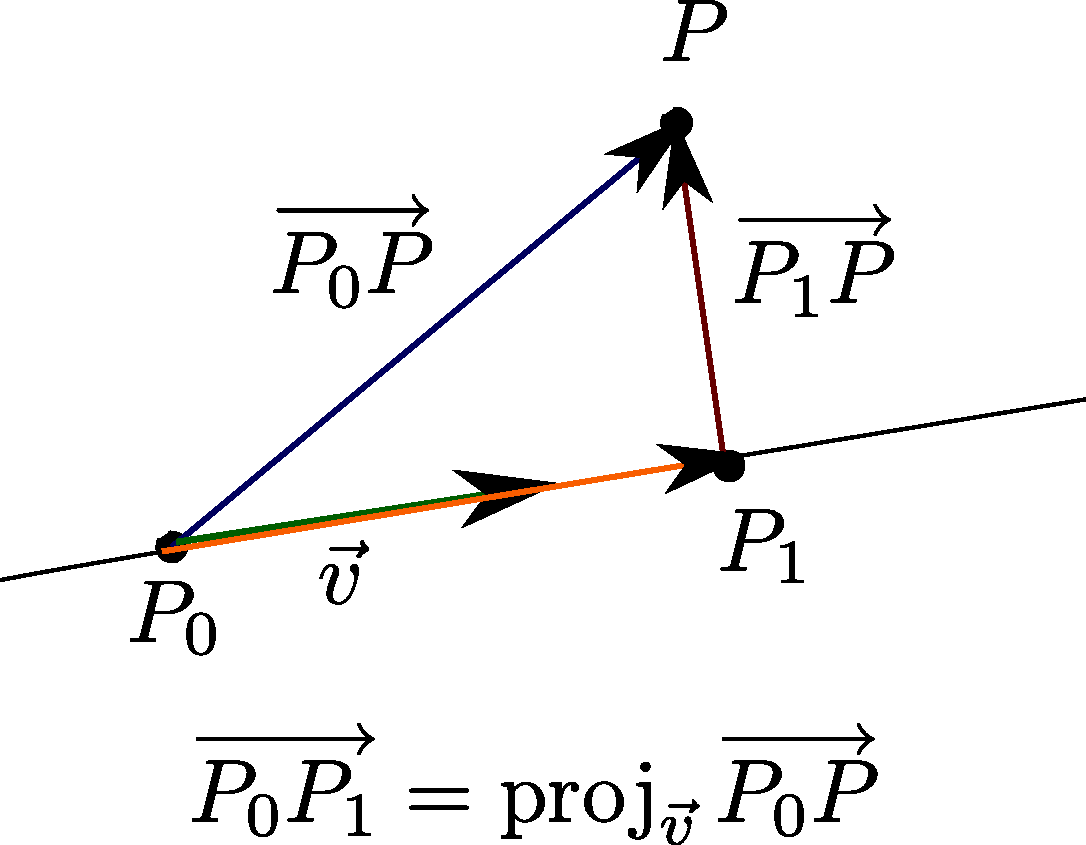
\includegraphics[width=0.7\columnwidth]{WS3-3}
\end{center}
\end{multicols}
We're given $\vec{v} = \langle 1,-1,0\rangle$, and we compute $\overrightarrow{P_0P}=\overrightarrow{OP}-\overrightarrow{OP_0} = \langle 1, 3, -2\rangle-\langle 2, 0, -1\rangle =\langle -1, 3, -1\rangle$. Since $\vec{v}\dotp \overrightarrow{P_0P} = 1(-1)+(-1)(3)+(0)(-1) = -4$ and $\len{\vec{v}}^2 = \vec{v}\dotp\vec{v} = 1^2+(-1)^2+0^2 = 2$, we have
\[
 \overrightarrow{P_0P_1} = \proj_{\vec{v}}\overrightarrow{P_0P} = \left(\frac{\vec{v}\dotp \overrightarrow{P_0P}}{\len{\vec{v}}^2}\right)\vec{v} = \frac{-4}{2}\langle 1, -1, 0\rangle = \langle -2, 2, 0\rangle.
\]
Since $\overrightarrow{P_0P_1} = \overrightarrow{OP_1}-\overrightarrow{OP_0}$, we have
\[
 \overrightarrow{OP_1} = \overrightarrow{OP_0}+\overrightarrow{P_0P_1} = \langle 2, 0, -1\rangle + \langle -2, 2, 0\rangle = \langle 0, 2, -1\rangle,
\]
and thus $P_1 = (0,2,-1)$. Finally, since $P_1$ is the closest point on our line to the point $P$ (as per the diagram above), the distance from the point $P$ to the line is the same as the distance from $P$ to $P_1$. Thus,
\[
 d = d(P,P_1) = \sqrt{(1-0)^2+(3-2)^2+(-2+(-1))^2} = \sqrt{1+1+1}=\sqrt{3}.
\]

{\bf Note:} if we wanted only the distance but didn't need to find the point $P_1$, we can notice (from -- guess what? -- the diagram!) that the distance from the point $P$ to the line is given by the length of the vector $\overrightarrow{P_1P}$, and that 
\[
\overrightarrow{P_1P} = \overrightarrow{P_0P}-\overrightarrow{P_0P_1} = \langle -1, 3, -1\rangle - \langle -2, 2, 0\rangle = \langle 1, 1,  -1\rangle,
\]
and thus $d = \len{\overrightarrow{P_1P}} = \sqrt{1^2+1^2+(-1)^2} = \sqrt{3}$.

\newpage


\item Find the distance between the skew lines 
\begin{align*}
 \ell_1(s) = \langle x,y,z\rangle & = \langle 1,2,1\rangle+s\langle 2,-1,1\rangle\\
 \ell_2(t) = \langle x,y,z\rangle & = \langle 3,3,3\rangle+t\langle 4,2,-1\rangle
\end{align*}
using the method of Example 47 in the text. 

\bigskip

Letting $P_1 = (1,2,1)$ and $P_2=(3,3,3)$ be the given points on the lines $\ell_1$ and $\ell_2$, respectively, we have the vector 
\[
 \vec{w} = \overrightarrow{P_1P_2} = \langle 2,1,2\rangle,
\]
which has its tail on $\ell_1$ and head on $\ell_2$. To compute the distance from $\ell_1$ to $\ell_2$, we need to determine the component of $\vec{w}$ that is perpendicular to both lines. We are given the direction vectors $\vec{v}_1 = \langle 2,-1,1\rangle$ and $\vec{v}_2 = \langle 4,2,-1\rangle$ for the two lines; since these vectors are parallel to their respective lines, the cross product
\[
 \vec{n} = \vec{v}_1\times\vec{v}_2 = \begin{vmatrix}\hat{\imath}&\hat{\jmath}&\hat{k}\\2&-1&1\\4&2&-1\end{vmatrix} = \langle -1, 6, 8\rangle
\]
must be perpendicular to both lines. (The notation $\vec{n}$ is used to indicate the fact that the two skew lines lie in parallel planes, both of which have the normal vector $\vec{n}$. Finding the distance between the two lines is thus reduced to finding the distance between the corresponding parallel planes.)

The desired distance is now given by the length of the projection of $\vec{w}$ onto $\vec{n}$. We have
\[
 d = \len{\operatorname{proj}_{\vec{n}}\vec{w}} = \frac{\abs{\vec{n}\dotp\vec{w}}}{\len{\vec{n}}} = \frac{-2+6+16}{\sqrt{1^2+6^2+8^2}} = \frac{20}{\sqrt{101}}.
\]
\end{enumerate}
  
\end{document}